\documentclass[../main.tex]{subfiles}

\begin{document}

\section{Introduction}

This section of the thesis describes the execution, results and conclusions of each individual study carried out. It is divided into two sections:

\begin{itemize}
    \item Simulation studies - taking simulated data and simulated algorithm results to analyse the impact of various cases on calculated measures.
    \item Real-World Data - taking a set of real world twitter data and analysing the ability of change detection algorithms to detect changes in the data compared with established ground truth change points.
\end{itemize}

\section{Simulation Studies}

The simulation studies carried out are intended to compare each of the measures against the set of criteria described in \autoref{meta analysis explainer}. The simulations are carried out according to the experiment descriptions previously explained, and the execution and results are presented here.

The scores given by `intermediate' metrics used to calculate final metrics (recall and precision for both F1 Score and BCubed F-Score) are also plotted for completeness, though they will not be subject to the result discussion.

\subsection{Dependence on Sample Size}
\label{sample size dependence}

Two of the experiments carried out in this thesis take particular note of sample size. Both involve increasing the sample size of the data, appending or prepending a number of points both prior to and following the ground truth change point. In each situation, a simulated algorithm detects a change $n$ points after the ground truth, simulating detection that is relevant, though slightly late, to ensure that there that the baseline metric value at $t = 0$ is not equal to $1$.

\begin{figure}[h]
    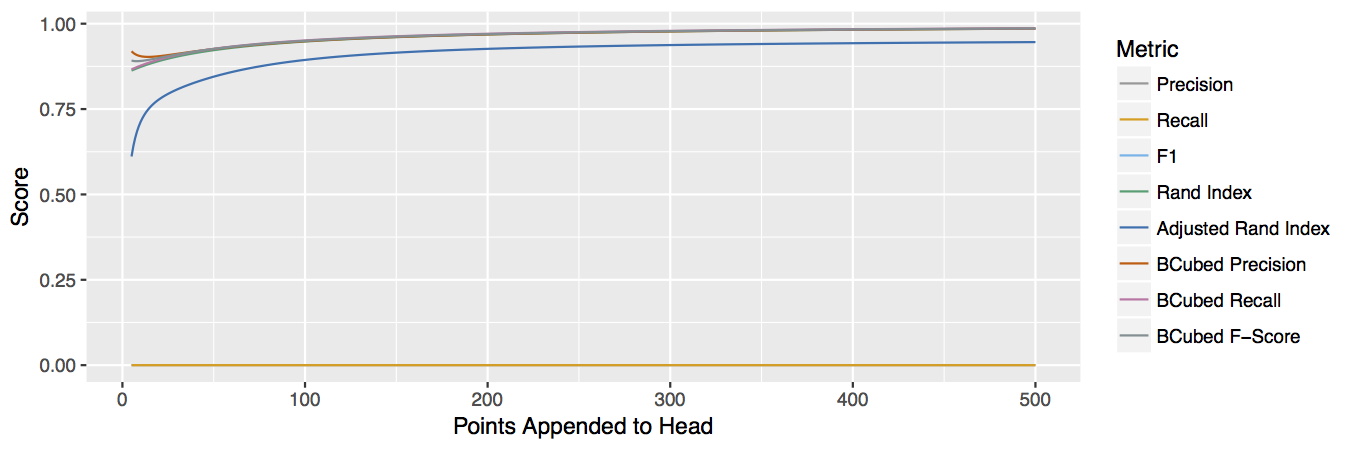
\includegraphics[width=\textwidth]{figures/Experiment1}
    \caption{Tail-Append Results Plot}
    \label{fig:Experiment1}
\end{figure}

\begin{figure}[h]
    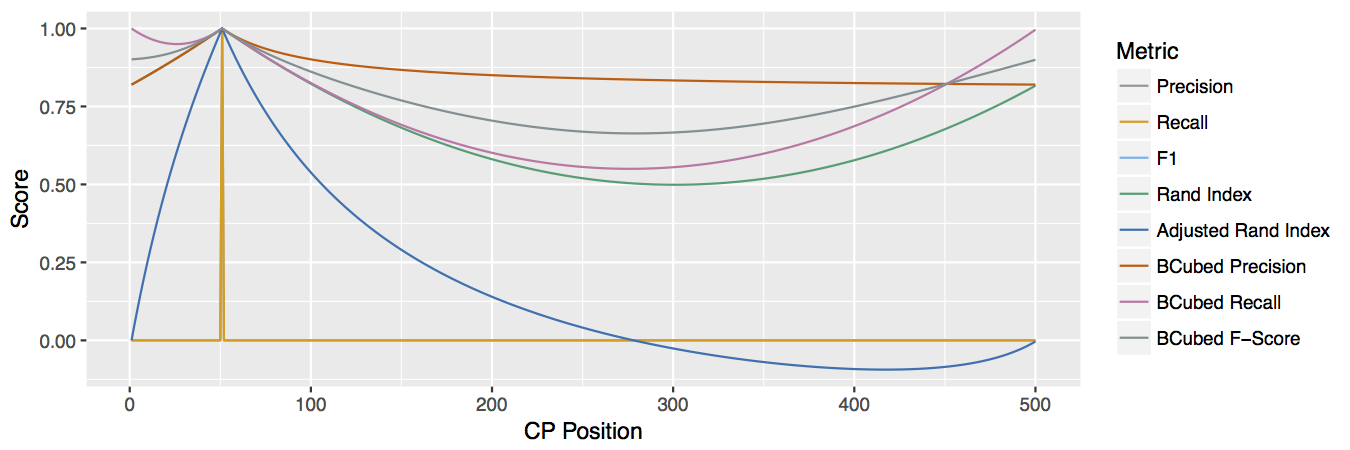
\includegraphics[width=\textwidth]{figures/Experiment4}
    \caption{Head-Prepend Results Plot}
    \label{fig:Experiment2}
\end{figure}

\autoref{fig:Experiment1} and \autoref{fig:Experiment2} show the results of this simulation study. \autoref{fig:Experiment2} demonstrates the value of metrics as the `head' of the data is increased, while \autoref{fig:Experiment1} demonstrates the value of metrics as the `tail' of the data is increased.

In this situation, we can see that both studies show a variation in metric score as the length of the data stream increases. For all of the clustering measures there is a clear increase in metric value as points are added. At $t=0$, the clustering metrics appear to correctly penalise for a late detection, though this penalty decreases as $t$ increases.

The Adjusted Rand Index shows a far more extreme temporal penalty for the change point detection, which increases sharply at the beginning of the experiment, before maintaining a rate of increase comparable to the other clustering measures.

The binary classification measures of Precision, Recall and F1 maintain a constant value of $0$ throughout the experiment, classifying the change point detection as a `missed' detection and penalising accordingly. For clarity, the hypotheses are again stated here:

\begin{hypothesis*}
    The measures will be affected in some way by additional points before the change point. It is also hypothesised that data set length will have an affect on the metric value.
\end{hypothesis*}

\begin{hypothesis*}
    The measures will be affected in some way by additional points after the change point. It is also hypothesised that data set length will have an affect on the metric value.
\end{hypothesis*}

\begin{nullhypothesis*}
    Neither additional points before a change point, nor data set length, will have an affect on the scores provided by evaluation metrics.
\end{nullhypothesis*}

\begin{nullhypothesis*}
    Neither additional points after a change point, nor data set length, will have an affect on the scores provided by evaluation metrics.
\end{nullhypothesis*}

For these experiments (1 \& 2) the null hypothesis $H_0$ is rejected, and the alternative hypothesis $H_1$ is accepted.

\subsection{Impact of Data Preceding and Following a Known Change Point}

The experiment run for this criteria is similar to those run in \autoref{sample size dependence}, but differs in one important manner: the size of the time series is maintained at a constant value throughout. As points are added to the `head' of the data set, points are removed from the `tail'. In practice, this serves to move both the true and computed change points through the time series.

\begin{figure}[h]
    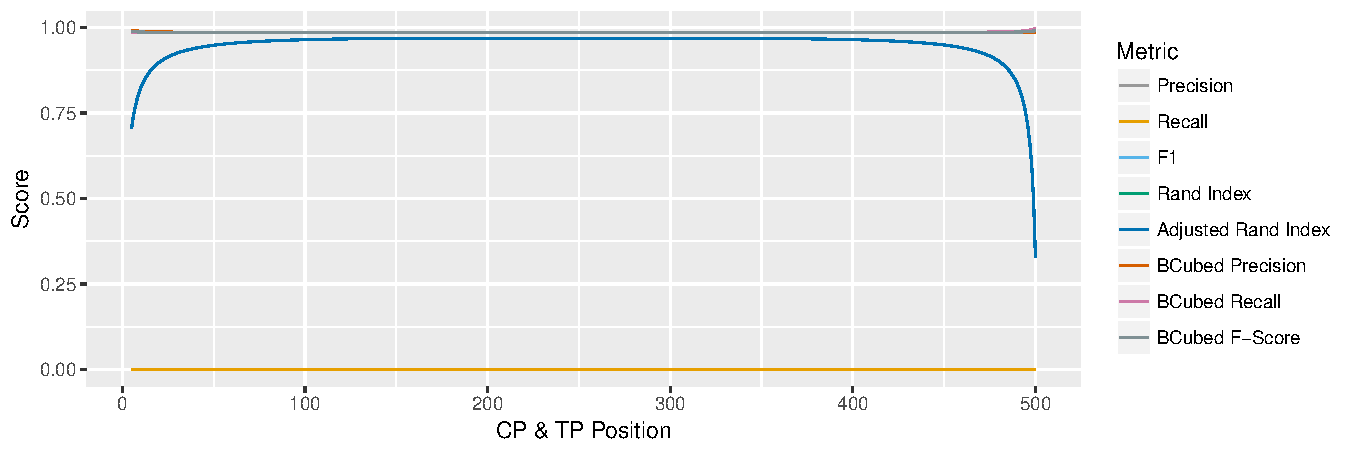
\includegraphics[width=\textwidth]{figures/Experiment2}
    \caption{Fixed Length Append/Prepend Results Plot}
    \label{fig:Experiment3}
\end{figure}

\autoref{fig:Experiment3} shows the results of the experiment. As with the previous experiment, the binary classification measures maintain a constant value of $0$, with variation only being shown by the clustering measures. It is interesting to note that the change in all clustering measures aside from Adjusted Rand Index is minimal, with an almost constant value being held throughout the experiment, aside from when the change points are at the extreme ends of the time series.

The Adjusted Rand Index exhibits behaviour unique to itself, with a value approaching 0 as the change points approach either end of time series. From position 150 to 350, the Adjusted Rand Index holds an almost constant value.

From these results it can be inferred that it is only the Adjusted Rand Index that is effected in any meaningful way by the position of the change point in a fixed length data set. For readability, the hypotheses are again stated here:

\begin{hypothesis*}
    The measures will be affected in some way by additional points before or after the change point. It is also hypothesised that data set length will have an affect on the metric value.
\end{hypothesis*}

\begin{nullhypothesis*}
    Neither additional points before or after a change point, nor data set length, will have an affect on the scores provided by evaluation metrics.
\end{nullhypothesis*}

For this experiment (3), the null hypothesis $H_0$ fails to be rejected for several measures. The only situation in which the alternative hypothesis $H_1$ holds is with the Adjusted Rand Index, which shows a considerable range in values when the change point is at the extreme ends of the time series.

\subsection{Temporal Penalty}

This is experiment makes use of a fixed length data set with a single, static, known change point. A computed change point is moved through the time series, beginning at the known change point, and ending at the end of the time series. \autoref{fig:Experiment4} shows a plot of the results of this experiment:

\begin{figure}[h]
    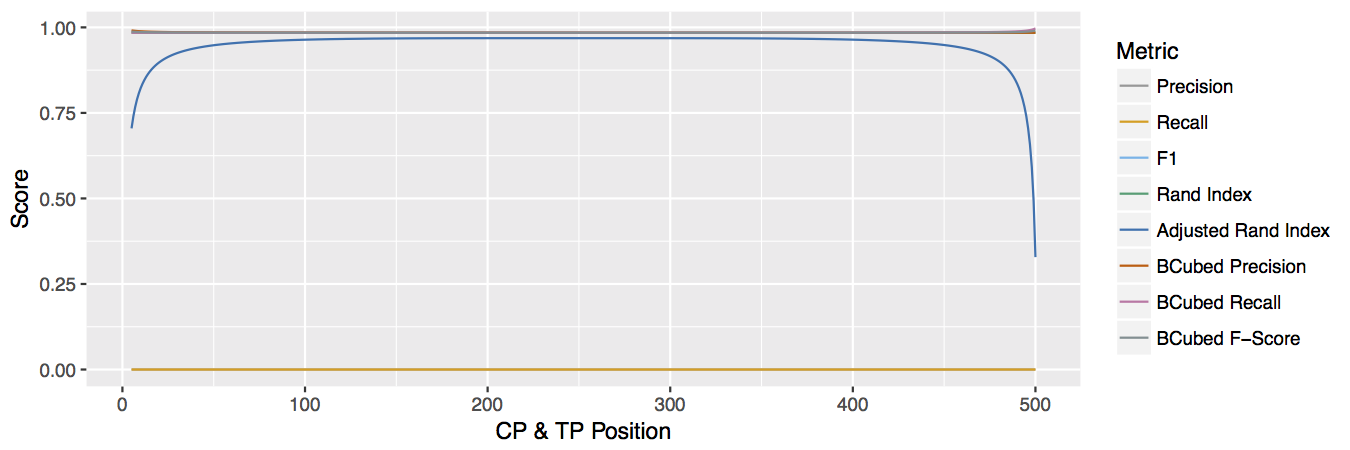
\includegraphics[width=\textwidth]{figures/Experiment3}
    \caption{Temporal Penalty Results Plot}
    \label{fig:Experiment4}
\end{figure}

At the start of the experiment, when the computed change point and the true change point are positioned such that there is an early detection, all of the scores except for BCubed Recall appear to penalise for this. When the ground truth and the computed change point are equal, all of the measures return a value of $1$ as expected. Once the computed change point is moved through the time series, the binary classification measures immediately return a value of $0$, showing that none of the change points in the series (a single change point, in this case) have been detected.

All of the clustering measure values decrease as the computed change point moves away from the ground truth change point, though exhibit some strange behaviour as the computed change point approaches the end of the time series. In all cases, the clustering measures show an increase in score as the computed point approaches the end of the time series, with the temporal penalty for a late detection reducing.

The Adjusted Rand Index once again exhibits behaviour unique to itself, dropping below $0$ at approximately $t=278$. This behaviour is expected from the Adjusted Rand Index, being that the adjusted nature of the metric (allowing for cluster classification occurring by chance) results in a metric capable of returning a value $<0$.

\pagebreak

For readability the hypotheses of this experiment are repeated here:

\begin{hypothesis*}
    One or more measures will incorrectly issue scores for a detected change point occurring various distances from the true change point.
\end{hypothesis*}

\begin{nullhypothesis*}
    All of the calculated metrics will correctly issue a penalty for late detections of a change point, in all instances.
\end{nullhypothesis*}

The results of this experiment (4) cause the null hypothesis $H_0$ to be rejected. All of the measures show some issue with the application of a temporal penalty for late detections, and indeed also show issues with crediting algorithms for early detections. In this case, the alternative hypothesis $H_1$ holds.

\subsection{Penalisation for False Positives}

This experiment utilised a fixed length time series with a single ground truth change point, and a single computed change point that equals the ground truth change point. Successive false positives are added to the time series, moving from left to right across the time series.

\autoref{fig:Experiment5} shows the results of the experiment, with the score provided by each metric plotted against the number of false positives present in the data stream.

\begin{figure}[h]
    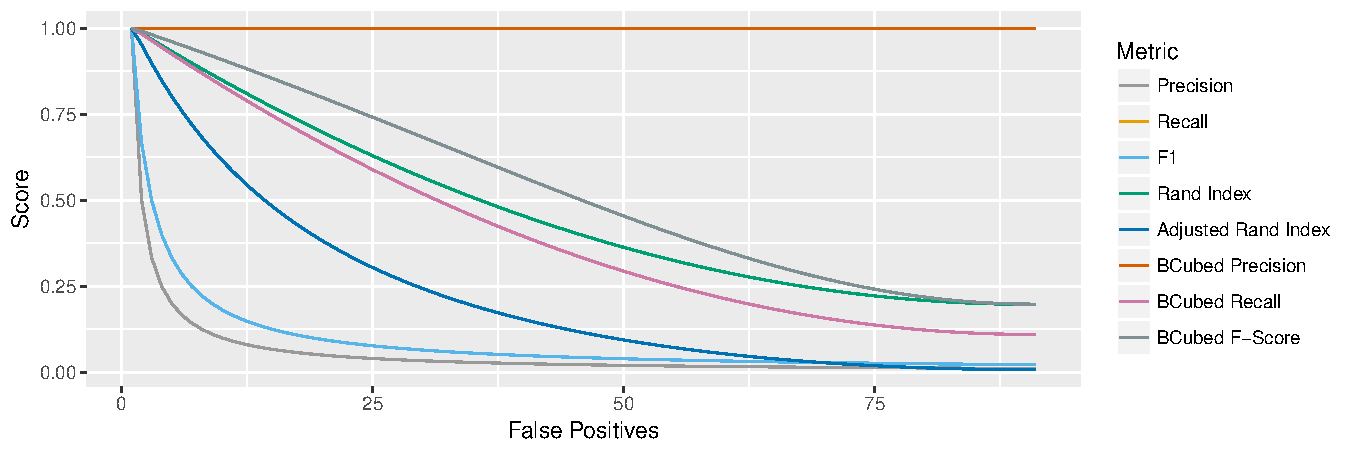
\includegraphics[width=\textwidth]{figures/Experiment5}
    \caption{False Positives Results Plot}
    \label{fig:Experiment5}
\end{figure}

The results of this experiment show that almost all of the metrics behave in a similar fashion. The binary classification measure of Recall maintains a value of $1$, while all of the other measures show a precipitous drop in score as the initial false positives are added. Precision and F1 scores for binary classification drop sharply, while the measures for clustering show a more gentle decrease in score. The Rand Index and BCubed F-Score end the experiment at approximately the same value, while the Adjusted Rand Index, F1 Score and Binary Classification Precision metrics also terminate at approximately the same value. For readability the hypotheses for this experiment are repeated here:

\begin{hypothesis*}
    The measures will not correctly issue penalties for false positive detections.
\end{hypothesis*}

\begin{nullhypothesis*}
    All of the metrics will correctly penalise for false positive detections in a time series.
\end{nullhypothesis*}

The results of this experiment cause the null hypothesis $H_0$ to hold, as all metrics behave correctly in this situation.

\subsection{Penalisation for False Negatives}

For this criteria evaluation, the experiment utilised a fixed length time series with multiple ground truth change points. As the experiment progressed, computed change points were added, equal to each of the ground truth change points. \autoref{fig:Experiment6} shows the results of the experiment, with the metric scores plotted against the number of false negatives present in the data stream.

\begin{figure}[h]
    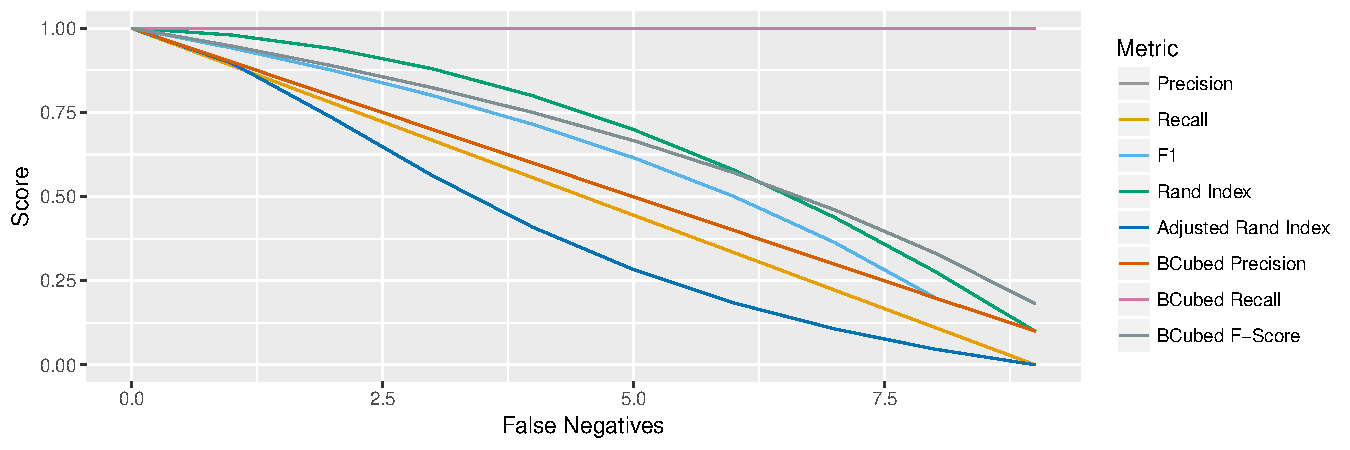
\includegraphics[width=\textwidth]{figures/Experiment6}
    \caption{False Negatives Results Plot}
    \label{fig:Experiment6}
\end{figure}

The vast majority of measures see a consistent decrease in returned score as the number of false negatives increases. Indeed, once all of the ground truth change points have been correctly detected, all of the metrics return a score of $1$. Only the Adjusted Rand Index returns a score of $0$ after $10$ false negatives are found in the data stream. As expected, BCubed Recall remained at a value of $1$ for the duration of the experiment. For readability, the hypotheses for this experiment are repeated:

\begin{hypothesis*}
    The measures will not appear to correctly increase in value as false negatives are removed from the data set - showing instead inconsistent behaviour.
\end{hypothesis*}

\begin{nullhypothesis*}
    Removing false negative results will result in a linear increase in score from each metric.
\end{nullhypothesis*}

The results of this experiment cause the null hypothesis $H_0$ to be rejected, and the alternative hypothesis $H_1$ to hold.

\subsection{Number of Change Points in Fixed Length Data Stream}

This experiment adds change points to a data stream by `lifting' slices of the data stream - adding a value to them to create two change points. This is carried out multiple times, each time adding two ground truth change points, and two computed change points 3 time units after the ground truth change points. \autoref{fig:Experiment7} shows the results of this experiment, plotting the score returned by the metric against the number of change points in the stream.

\begin{figure}[h]
    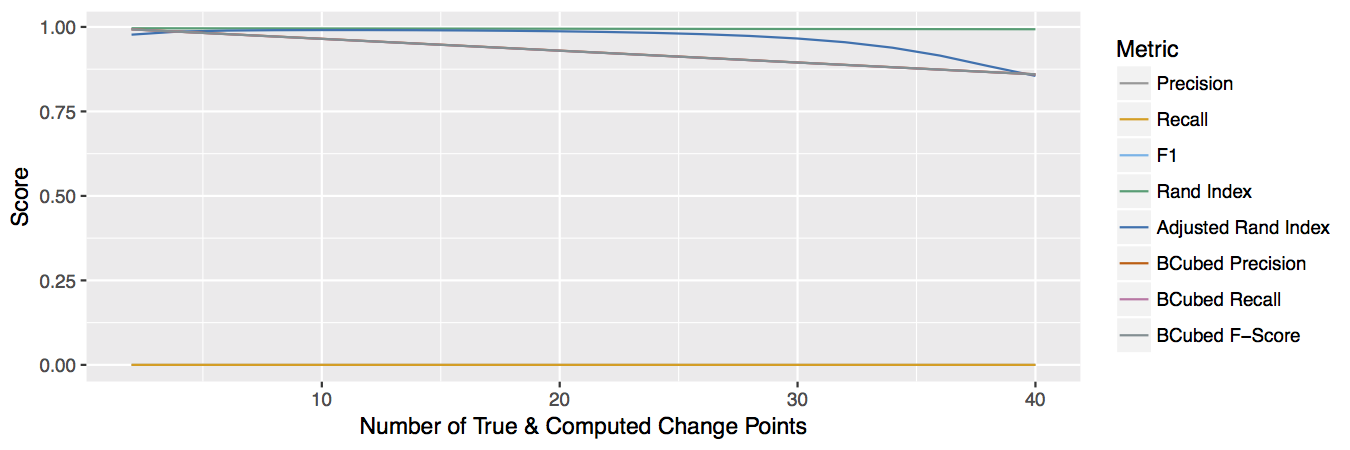
\includegraphics[width=\textwidth]{figures/Experiment8}
    \caption{Change Point Density (Fixed Length) Results Plot}
    \label{fig:Experiment7}
\end{figure}

The results of this experiment show a drop in score provided by the Adjusted Rand Index and BCubed F-Score. The BCubed F-Score shows a linear rate of decline as change points are added to the stream, while the Adjusted Rand Index shows an increase in downward velocity towards the end of the experiment. All of the other metrics maintained a constant value of either $1$ or $0$, as expected. The hypotheses for this experiment are as follows:

\begin{hypothesis*}
    The measures will be affected in some way by change point density and data set length, showing an increase or decrease in score value as density and length increases.
\end{hypothesis*}

\begin{nullhypothesis*}
    Metrics will be unaffected by change point density in a time series, nor will they be affected for changes in time series length.
\end{nullhypothesis*}

The results of this experiment cause the alternative hypothesis $H_1$ to be accepted, and thus the null hypothesis $H_0$ is rejected.

\subsection{Number of Change Points in Variable Length Data Stream}

This final experiment is similar to the previous one, in that it increases the number of change points in a data stream. However, the difference here is that in this case, data is appended to the data stream, also increasing the length of the stream as each successive change point is added. The results of this experiment are shown in \autoref{fig:Experiment8}:

\begin{figure}[H]
    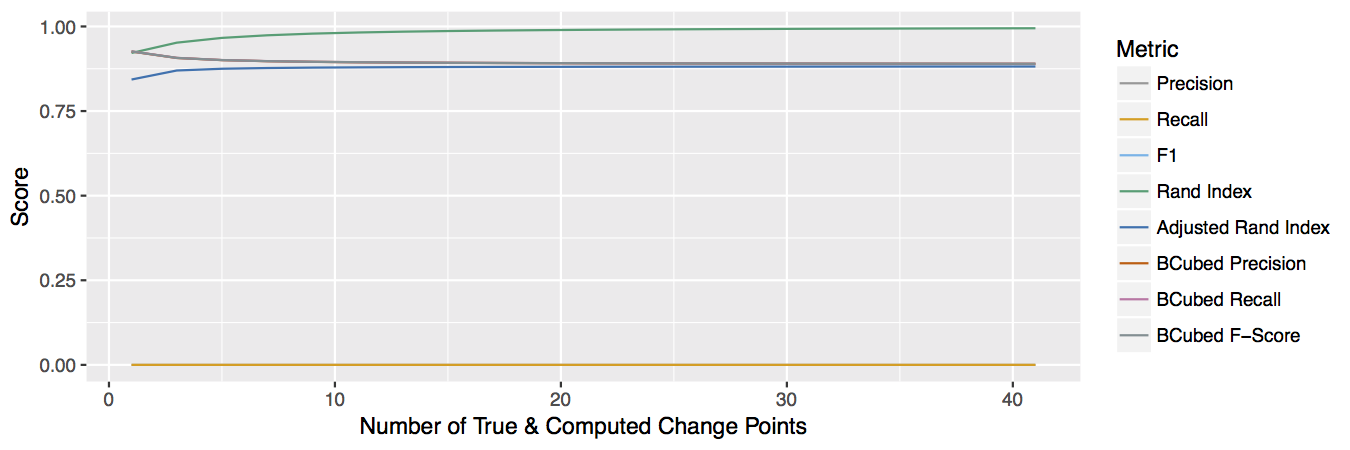
\includegraphics[width=\textwidth]{figures/Experiment7}
    \caption{Change Point Density (Variable Length) Results Plot}
    \label{fig:Experiment8}
\end{figure}

The results of the experiment show some interesting behaviour in the Rand Index, Adjusted Rand Index and BCubed F-Score metrics. The Rand index and the Adjusted Rand Index increase in value as data points and change points are added to the time series, while the BCubed F-Score decreases in value. The Adjusted Rand Index begins at a slightly lower level than the Rand Index and BCubed F-Score metrics, while the Rand Index and BCubed F-Score metrics diverge almost immediately.

Aside from the large change in score value at the beginning of the experiment, the change in value for the Rand Index, Adjusted Rand Index and BCubed F-Score metrics is small. The hypotheses for this experiment are as follows:

\begin{hypothesis*}
    The measures will be affected in some way by changes in change point density. The hypothesis is that the value of the measures will increase or decrease as change point density increases.
\end{hypothesis*}

\begin{nullhypothesis*}
    Metrics will be unaffected by change point density, maintaining a constant value.
\end{nullhypothesis*}

In this experiment, the alternative hypothesis $H_1$ holds, allowing for the rejection of the null hypothesis $H_0$.

\section{Functional Requirements}

This research was completed by carrying out a requirements elicitation process with the lead developer of the host company. Conversations and discussions were had throughout the execution of this project, and what follows is a listing of functional requirements that were gleaned as a part of this process:

\begin{description}
    \item[R1] The approach should not rely on arbitrary threshold values. It instead should adapt to the data that it is analysing.
    \item[R2] False positives should not be considered wholly harmful. The consequence of a false positive in production is only that a notification is sent. That said, false positives should be kept to a reasonable level.
    \item[R3] Late detections should be considered failure cases. Late detections are not useful to clients using the production system, as prompt detections are needed for effective damage control in situations where increased conversation volume is caused by a PR crisis.
    \item[R4] Similarly, false negatives should also be considered failure cases. False negatives are defined as when the algorithm fails to flag a change point that would have been flagged by manual, by-eye analysis. False negatives prevent clients from acting upon changes in conversation volume in a timely manner.
    \item[R5] The approach in it's first iteration should operate on conversation volume metrics provided by Brandmonitor, but should be extensible such that it can also be applied to other metrics.
\end{description}

These requirements were then used, along with the results of the simulation studies, to evaluate if one or more of the measures are best suited for evaluating the change detection methods used in the real-world data analysis study. A full summary of how the measures performed when compared with these requirements can be found in \autoref{conclusions}

\section{Real-World Data Analysis}

As described in \autoref{real world explainer}, this experiment executed change detection algorithms against sets of real-world conversation volume data taken from online social media, print, TV and radio sources. The data was gathered and filtered to be relevant to certain brands (again, as listed in \autoref{real world explainer}) and then annotated with ground truth change points by social media analysts from the host organisation. The ground truth annotations can be found in \autoref{groundtruth}.

What follows is the results of that study. For each data set, the scores provided by the evaluation measures are tabulated and provided in \autoref{fullscores}. The highest score(s) for each measure are highlighted for easy comparison and readability. Further discussion of the results and the extraction of conclusions will can be found in \autoref{results} and \autoref{conclusions}.

\pagebreak

The final plots, including detected change points by each algorithm can also be found in \autoref{changeplots}.

Analysis of the raw data used for \autoref{fig:PrettyPlot} shows that while there is a consensus on the best algorithm, some metrics provide higher scores for algorithms that perform objectively worse than others, when compared through by-eye analysis of the change point plots. Binary classification scores are universally low for all data sets.

\begin{figure}[h]
    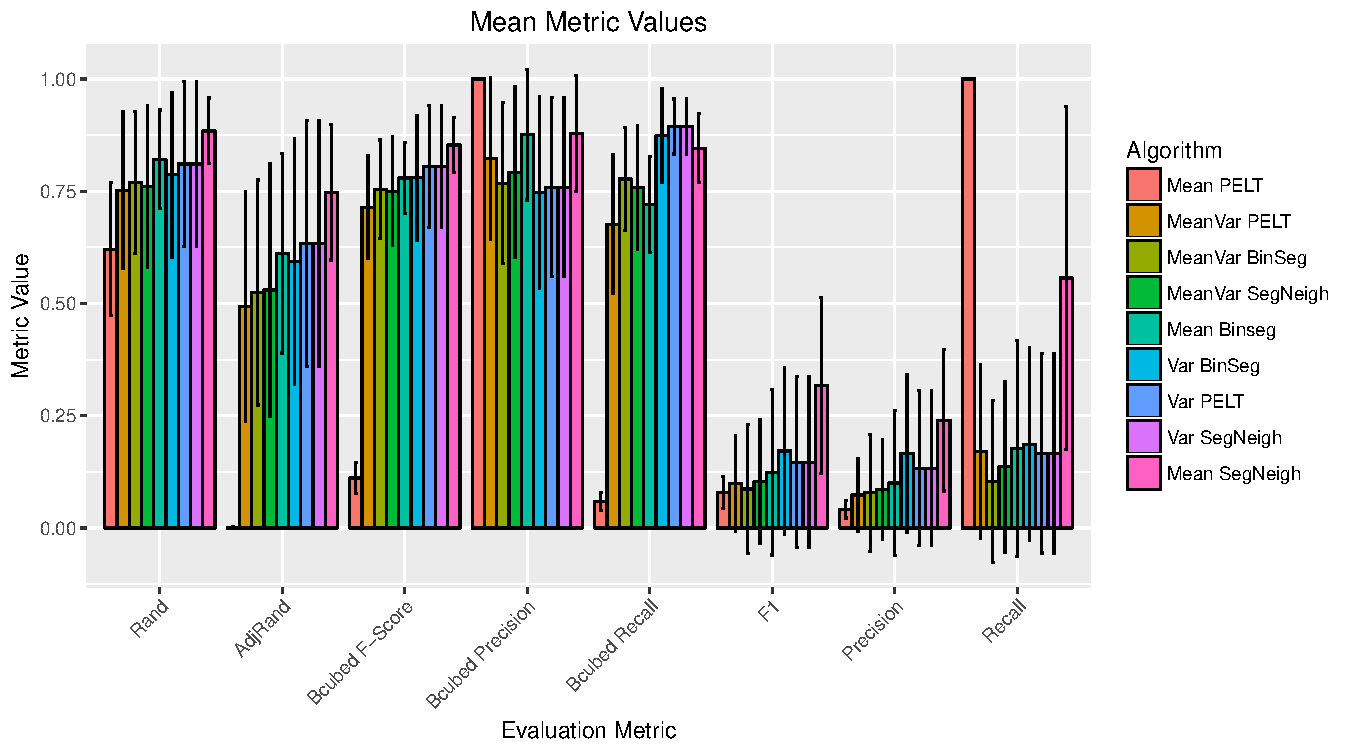
\includegraphics[width=\textwidth]{figures/PrettyPlot2}
    \caption{Average scores across all real-world data scenarios}
    \label{fig:PrettyPlot}
\end{figure}

\autoref{fig:PrettyPlot} shows a plot of average score values across all real-world data sets, from each algorithm. The error bars are drawn to show 1 standard deviation of error.

Taking the mean metric score for each algorithm across all of the experiments, we can rank the algorithms as follows, using the four main metrics that this research was focussing on:

\begin{table}[h]
\centering
\begin{tabular}{@{}rcccc@{}}
\toprule
\textbf{Rank} & \textbf{F1 Score} & \textbf{Rand Index} & \textbf{Adjusted Rand Index} & \textbf{BCubed F-Score} \\ \midrule
1 & Mean Segneigh & Mean SegNeigh & Mean SegNeigh & Mean SegNeigh \\
2 & Var BinSeg & Mean BinSeg & Mean BinSeg & Var PELT \\
3 & Var PELT & Var PELT & Var PELT & Var SegNeigh \\
4 & Var SegNeigh & Var SegNeigh & Var SegNeigh & Var BinSeg \\
5 & Mean BinSeg & Var BinSeg & Var BinSeg & Mean BinSeg \\
6 & MeanVar SegNeigh & MeanVar BinSeg & MeanVar BinSeg & MeanVar BinSeg \\
7 & Meanvar PELT & MeanVar SegNeigh & MeanVar SegNeigh & MeanVar SegNeigh \\
8 & MeanVar BinSeg & MeanVar PELT & MeanVar PELT & MeanVar PELT \\
9 & Mean PELT & Mean PELT & Mean PELT & Mean PELT \\ \bottomrule
\end{tabular}
\caption{Algorithm Rankings}
\label{tab:rankings}
\end{table}

Here it is clear that while there appears to be a consensus on the `best' algorithm in this limited trial, the remaining rankings vary somewhat. In order to analyse this, the \emph{Kendall's Tau} coefficient of ranking correlation is utilised \cite{KENDALL1938}. This measure produces values of 1 for identical rankings, and -1 for fully different rankings. The results of this calculation are shown in \autoref{tab:tau}.

\begin{table}[h]
\centering
\resizebox{\textwidth}{!}{%
\begin{tabular}{@{}rcccc@{}}
\toprule
\multicolumn{1}{l}{} & \textbf{F1 Ranks} & \textbf{\begin{tabular}[c]{@{}c@{}}Rand Index\\ Ranks\end{tabular}} & \textbf{\begin{tabular}[c]{@{}c@{}}Adjusted Rand\\ Index Ranks\end{tabular}} & \textbf{\begin{tabular}[c]{@{}c@{}}BCubed F-Score\\ Ranks\end{tabular}} \\ \midrule
\textbf{F1 Ranks} &  & 0.278 & 0.278 & 0.778 \\
\textbf{Rand Index Ranks} & 0.278 &  & 1 & 0.278 \\
\textbf{Adjusted Rand Index Ranks} & 0.278 & 1 &  & 0.278 \\
\textbf{BCubed F-Score Ranks} & 0.778 & 0.278 & 0.278 &  \\ \bottomrule
\end{tabular}%
}
\caption{Calculated Kendall's Tau values between pairs of rankings}
\label{tab:tau}
\end{table}

With these values in \autoref{tab:tau}, for each pair we can test the null hypothesis $H_0$ that $\tau = 0$ and there is no correlation between the rankings by computing the $p-value$ for each $\tau$. This gives results shown in \autoref{tab:pval}.

\begin{table}[h]
\centering
\resizebox{\textwidth}{!}{%
\begin{tabular}{@{}rcccc@{}}
\toprule
\multicolumn{1}{l}{} & \textbf{F1 Ranks} & \textbf{\begin{tabular}[c]{@{}c@{}}Rand Index\\ Ranks\end{tabular}} & \textbf{\begin{tabular}[c]{@{}c@{}}Adjusted Rand\\ Index Ranks\end{tabular}} & \textbf{\begin{tabular}[c]{@{}c@{}}BCubed F-Score\\ Ranks\end{tabular}} \\ \midrule
\textbf{F1 Ranks} &  & 0.3585 & 0.3585 & 0.002425 \\
\textbf{Rand Index Ranks} & 0.3585 &  & $5.51\times 10^{-6}$ & 0.3585 \\
\textbf{Adjusted Rand Index Ranks} & 0.3585 & $5.51\times 10^{-6}$ &  & 0.3585 \\
\textbf{BCubed F-Score Ranks} & 0.002425 & 0.3585 & 0.3585 &  \\ \bottomrule
\end{tabular}%
}
\caption{Calculated $p$ values for Kendall's Tau tests}
\label{tab:pval}
\end{table}

The values shown in \autoref{tab:pval} demonstrate that for the comparison of the rankings provided for F1 and BCubed F-Score, we can reject the null hypothesis $H_0$ that they are uncorrelated, with a 95\% confidence interval, as $p < 0.05$. Similarly, we can reject the null hypothesis for the ranks provided by the Rand Index and Adjusted Rand Index, with a confidence interval of 95\%, as $p < 0.05$. This is not unexpected, as the Adjusted Rand Index is derived from the classic Rand Index, and in the case of these experiments we would not expect to see any deviation in rankings provided. The other pairs of rankings show a $p$ value of $> 0.05$ and as such, the null hypothesis $H_0$ that these ranks are not correlated holds, with a 95\% confidence interval.

\end{document}